\documentclass[12pt,openany]{book}
\usepackage{lmodern}
\usepackage{amssymb,amsmath}
\usepackage{ifxetex,ifluatex}
\usepackage{fixltx2e} % provides \textsubscript
\ifnum 0\ifxetex 1\fi\ifluatex 1\fi=0 % if pdftex
  \usepackage[T1]{fontenc}
  \usepackage[utf8]{inputenc}
\else % if luatex or xelatex
  \ifxetex
    \usepackage{mathspec}
  \else
    \usepackage{fontspec}
  \fi
  \defaultfontfeatures{Ligatures=TeX,Scale=MatchLowercase}
\fi
% use upquote if available, for straight quotes in verbatim environments
\IfFileExists{upquote.sty}{\usepackage{upquote}}{}
% use microtype if available
\IfFileExists{microtype.sty}{%
\usepackage{microtype}
\UseMicrotypeSet[protrusion]{basicmath} % disable protrusion for tt fonts
}{}
\usepackage[margin=1in]{geometry}
\usepackage{hyperref}
\hypersetup{unicode=true,
            pdftitle={Analysis of the automobile-loss-prediction dataset},
            pdfauthor={Jared Musil \& Jake McNair},
            pdfborder={0 0 0},
            breaklinks=true}
\urlstyle{same}  % don't use monospace font for urls
\usepackage{natbib}
\bibliographystyle{apalike}
\usepackage{longtable,booktabs}
\usepackage{graphicx,grffile}
\makeatletter
\def\maxwidth{\ifdim\Gin@nat@width>\linewidth\linewidth\else\Gin@nat@width\fi}
\def\maxheight{\ifdim\Gin@nat@height>\textheight\textheight\else\Gin@nat@height\fi}
\makeatother
% Scale images if necessary, so that they will not overflow the page
% margins by default, and it is still possible to overwrite the defaults
% using explicit options in \includegraphics[width, height, ...]{}
\setkeys{Gin}{width=\maxwidth,height=\maxheight,keepaspectratio}
\IfFileExists{parskip.sty}{%
\usepackage{parskip}
}{% else
\setlength{\parindent}{0pt}
\setlength{\parskip}{6pt plus 2pt minus 1pt}
}
\setlength{\emergencystretch}{3em}  % prevent overfull lines
\providecommand{\tightlist}{%
  \setlength{\itemsep}{0pt}\setlength{\parskip}{0pt}}
\setcounter{secnumdepth}{5}
% Redefines (sub)paragraphs to behave more like sections
\ifx\paragraph\undefined\else
\let\oldparagraph\paragraph
\renewcommand{\paragraph}[1]{\oldparagraph{#1}\mbox{}}
\fi
\ifx\subparagraph\undefined\else
\let\oldsubparagraph\subparagraph
\renewcommand{\subparagraph}[1]{\oldsubparagraph{#1}\mbox{}}
\fi

%%% Use protect on footnotes to avoid problems with footnotes in titles
\let\rmarkdownfootnote\footnote%
\def\footnote{\protect\rmarkdownfootnote}

%%% Change title format to be more compact
\usepackage{titling}

% Create subtitle command for use in maketitle
\newcommand{\subtitle}[1]{
  \posttitle{
    \begin{center}\large#1\end{center}
    }
}

\setlength{\droptitle}{-2em}
  \title{Analysis of the ``automobile-loss-prediction'' dataset}
  \pretitle{\vspace{\droptitle}\centering\huge}
  \posttitle{\par}
\subtitle{Illinois State University - ACC 471 - Final Report}
  \author{Jared Musil \& Jake McNair}
  \preauthor{\centering\large\emph}
  \postauthor{\par}
  \predate{\centering\large\emph}
  \postdate{\par}
  \date{2017-11-29}

\usepackage{booktabs}
\usepackage{amsthm}
\makeatletter
\def\thm@space@setup{%
  \thm@preskip=8pt plus 2pt minus 4pt
  \thm@postskip=\thm@preskip
}
\makeatother

\begin{document}
\maketitle

{
\setcounter{tocdepth}{1}
\tableofcontents
}
\chapter{Introduction}\label{intro}

The ability to utilize analytics to predict automobiele lossess is a
area of active research and application throughout the insurance and
fin-tech industries. All of the ``big four'' US domiciled auto insurrers
being State Farm, Geico, Allstate, and Progressive are actively engaging
in research to operationalize analytical models to increase operational
efficency. {[}citation needed\ldots{}{]}. This dataset is representitive
of claims data common to all of these auto insurance providers, and the
industry at large.

From a consumer standpoint, this has the potential to reduce average
claim times, reduce premium costs, and improve claims decisions (total
loss, not total loss).

Throughout this report, the columns of our dataset will be refered to as
factors, and the rows of our dataset will be refered to as reccords.
This is because it follows the terminology used by the R statistical
programming language, which was the analytical tool used in this report.
This was chosen to allow for reproducable research and full transparency
of the methods used to arrive at our conclusions. The code itself has
been omitted from the report for brevity, but is available for review
and reuse at the following URL:
\url{https://github.com/jaredmusil/acc471-final-report}

\chapter{Problem Description}\label{problem-description}

This data set consists of three types of entities: (a) the specification
of an auto in terms of various characteristics, (b) its assigned
insurance risk rating, (c) its normalized losses in use as compared to
other cars. The second rating corresponds to the degree to which the
auto is more risky than its price indicates. Cars are initially assigned
a risk factor symbol associated with its price. Then, if it is more
risky (or less), this symbol is adjusted by moving it up (or down) the
scale. Actuarians call this process ``symboling''. A value of +3
indicates that the auto is risky, -3 that it is probably pretty safe.

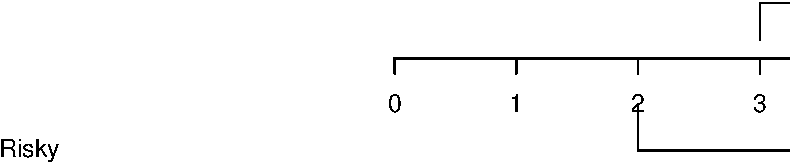
\includegraphics{bookdown-demo_files/figure-latex/risk-scale-1.pdf}

The third factor is the relative average loss payment per insured
vehicle year. This value is normalized for all autos within a particular
size classification (two-door small, station wagons, sports/speciality,
etc\ldots{}), and represents the average loss per car per year.

\chapter{Data}\label{data}

Before doing any analysis, the factors within the dataset were first
checked for missing or invalid data. The individual factors can be
described as follows: 15 continuous, 10 nominal, and 1 integer.

Seven of the factors contained missing or improperly coded data. In this
dataset in partular, all missing data has been coded with the value of
\texttt{?}. In all cases below, the records containing the missing data
have been removed.

\begin{longtable}[]{@{}lll@{}}
\toprule
Index & Factor & Number of records missing a value\tabularnewline
\midrule
\endhead
2 & normalized-losses & 41\tabularnewline
6 & num-of-doors & 2\tabularnewline
19 & bore & 4\tabularnewline
20 & stroke & 4\tabularnewline
22 & horsepower & 2\tabularnewline
23 & peak-rpm & 2\tabularnewline
26 & price & 4\tabularnewline
\bottomrule
\end{longtable}

Of the original 205 records, X were removed because they contained
missing data for the \texttt{normalized-lossess} factor, which was coded
as a \texttt{?}. This resulted in a dataset of 164 records of clean
data. No other factors needed cleaning up, as the data was properly
coded for each record.

\begin{table}

\caption{\label{tab:data-dictionary}Data Dictionary - Initial}
\centering
\begin{tabular}[t]{rlll}
\toprule
N & Description & Values & Keep\\
\midrule
1 & symboling & -3, -2, -1, 0, 1, 2, 3 & No\\
2 & normalized-losses & continuous from [65 to 256] & Yes\\
3 & make & alfa-romero, audi, bmw, chevrolet, dodge, honda, isuzu, jaguar, mazda, mercedes-benz, mercury, mitsubishi, nissan, peugot, plymouth, porsche, mitsubishi, nissan, peugot, plymouth, porsche, renault, saab, subaru, toyota, volkswagen, volvo & Yes\\
4 & fuel-type & diesel, gas & Yes\\
5 & aspiration & std, turbo & Yes\\
\addlinespace
6 & num-of-doors & four, two & Yes\\
7 & body-style & hardtop, wagon, sedan, hatchback, convertible & Yes\\
8 & drive-wheels & 4wd, fwd, rwd. & Yes\\
9 & engine-location & front, rear & Yes\\
10 & wheel-base & continuous from [86.6 to 120.9] & Yes\\
\addlinespace
11 & length & continuous from [141.1 to 208.1] & Yes\\
12 & width & continuous from [60.3 to 72.3] & Yes\\
13 & height & continuous from [47.8 to 59.8] & Yes\\
14 & curb-weight: & continuous from [1488 to 4066] & Yes\\
15 & engine-type & dohc, dohcv, l, ohc, ohcf, ohcv, rotor & Yes\\
\addlinespace
16 & num-of-cylinders & eight, five, four, six, three, twelve, two & Yes\\
17 & engine-size & continuous from [61 to 326] & Yes\\
18 & fuel-system & 1bbl, 2bbl, 4bbl, idi, mfi, mpfi, spdi, spfi & Yes\\
19 & bore & continuous from [2.54 to 3.94] & Yes\\
20 & stroke & continuous from [2.07 to 4.17] & Yes\\
\addlinespace
21 & compression-ratio & continuous from [7 to 23] & Yes\\
22 & horsepower & continuous from [48 to 288] & Yes\\
23 & peak-rpm & continuous from [4,150 to 6,600] & Yes\\
24 & city-mpg & continuous from [13 to 49] & Yes\\
25 & highway-mpg & continuous from [16 to 54] & Yes\\
26 & price & continuous from [5,118 to 45,400] & Yes\\
\bottomrule
\end{tabular}
\end{table}

Of these factors, 10 of the initial 26 were removed, resulting in the 16
factors that will be used in analysis. These factors are noted in green
in \texttt{Keep} column of the above table.

The objective factor in the dataset is determined to be
\texttt{symboling}.

Next, the data was partitioned into three groups named \emph{training},
\emph{test}, and \emph{validation}. This was

\begin{verbatim}
##        X1                X2            X3          X4          X5     
##  Min.   :-2.0000   Min.   : 65   toyota :31   diesel: 15   std  :136  
##  1st Qu.: 0.0000   1st Qu.: 94   nissan :18   gas   :149   turbo: 28  
##  Median : 1.0000   Median :115   mazda  :15                           
##  Mean   : 0.7927   Mean   :122   honda  :13                           
##  3rd Qu.: 2.0000   3rd Qu.:150   subaru :12                           
##  Max.   : 3.0000   Max.   :256   volvo  :11                           
##                                  (Other):64                           
##     X6               X7       X8          X9           X10        
##  ?   : 1   convertible: 2   4wd:  8   front:164   Min.   : 86.60  
##  four:95   hardtop    : 5   fwd:106               1st Qu.: 94.50  
##  two :68   hatchback  :60   rwd: 50               Median : 96.55  
##            sedan      :80                         Mean   : 98.16  
##            wagon      :17                         3rd Qu.:100.40  
##                                                   Max.   :115.60  
##                                                                   
##       X11             X12            X13             X14          X15     
##  Min.   :141.1   Min.   :60.3   Min.   :49.40   Min.   :1488   dohc :  8  
##  1st Qu.:165.7   1st Qu.:64.0   1st Qu.:52.00   1st Qu.:2091   l    :  8  
##  Median :172.0   Median :65.4   Median :54.10   Median :2368   ohc  :124  
##  Mean   :172.2   Mean   :65.6   Mean   :53.77   Mean   :2458   ohcf : 12  
##  3rd Qu.:177.8   3rd Qu.:66.5   3rd Qu.:55.50   3rd Qu.:2786   ohcv :  8  
##  Max.   :202.6   Max.   :71.7   Max.   :59.80   Max.   :4066   rotor:  4  
##                                                                           
##     X16           X17          X18          X19          X20    
##  eight:  1   Min.   : 61.0   1bbl:11   3.62   :20   3.03   :14  
##  five :  7   1st Qu.: 97.0   2bbl:63   3.15   :15   3.15   :14  
##  four :137   Median :109.0   4bbl: 3   3.19   :15   3.4    :13  
##  six  : 14   Mean   :118.0   idi :15   2.97   :12   3.23   :12  
##  three:  1   3rd Qu.:131.8   mfi : 1   3.03   :10   2.64   :11  
##  two  :  4   Max.   :258.0   mpfi:66   2.91   : 7   3.29   : 9  
##                              spdi: 5   (Other):85   (Other):91  
##       X21             X22              X23            X24       
##  Min.   : 7.00   Min.   : 48.00   Min.   :4150   Min.   :15.00  
##  1st Qu.: 8.70   1st Qu.: 69.00   1st Qu.:4800   1st Qu.:22.00  
##  Median : 9.00   Median : 91.00   Median :5200   Median :26.00  
##  Mean   :10.13   Mean   : 96.21   Mean   :5138   Mean   :26.27  
##  3rd Qu.: 9.40   3rd Qu.:114.00   3rd Qu.:5500   3rd Qu.:31.00  
##  Max.   :23.00   Max.   :200.00   Max.   :6600   Max.   :49.00  
##                                                                 
##       X25             X26       
##  Min.   :18.00   Min.   : 5118  
##  1st Qu.:28.00   1st Qu.: 7446  
##  Median :32.00   Median : 9268  
##  Mean   :31.85   Mean   :11467  
##  3rd Qu.:37.00   3rd Qu.:14559  
##  Max.   :54.00   Max.   :35056  
## 
\end{verbatim}

\chapter{Methods Used}\label{methods-used}

A number of analytical methods are available for use such as decision
trees, classification trees, regression, multiple-regression. Not all of
these techniques makes sense for our purpouses as they are used to
predict diffrent types of information.

We utilized \texttt{X} methods in our analysis, while setteling on
regression trees for our final reccomendation.

The main goal of our analysis is to predict how risky a particular car
is, and therefore Regression trees make the most sense.

\begin{figure}[htbp]
\centering
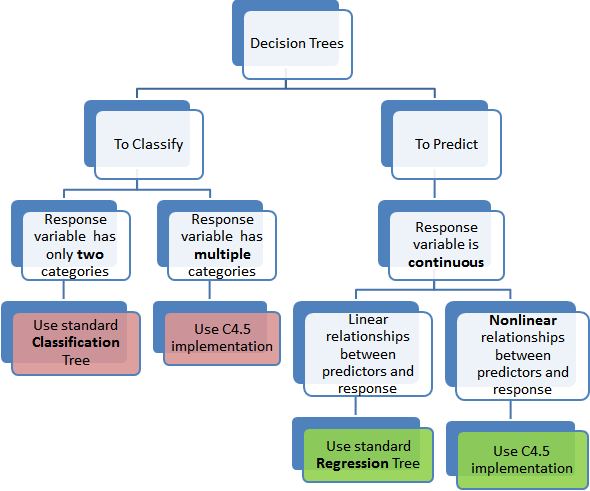
\includegraphics{img/04-decision-tree-flowchart.png}
\caption{\textbf{Source:}
\url{http://www.simafore.com/blog/bid/62482/2-main-differences-between-classification-and-regression-trees}}
\end{figure}

\chapter{Results}\label{results}

\ldots{}

\section{Regression Tree}\label{regression-tree}

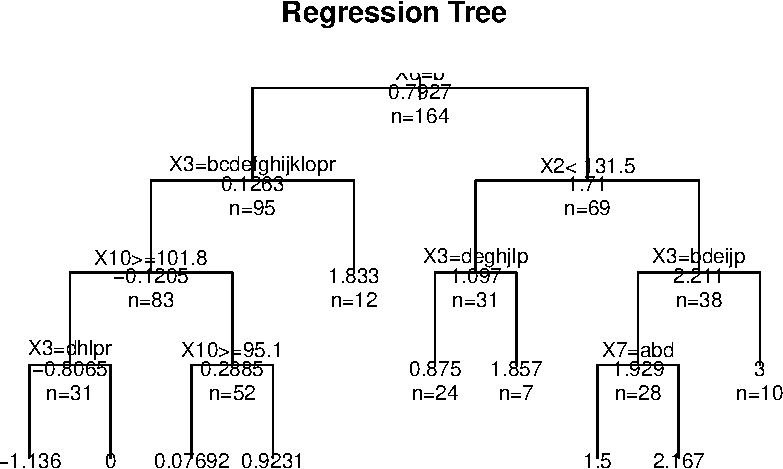
\includegraphics{bookdown-demo_files/figure-latex/regression-tree-1.pdf}

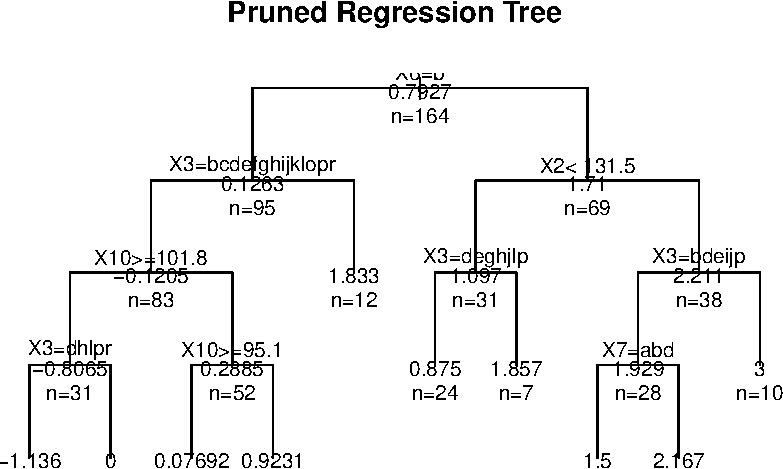
\includegraphics{bookdown-demo_files/figure-latex/regression-tree-pruned-1.pdf}

\ldots{}

\textbf{Lift Chart}

\ldots{}

\textbf{Decile Chart}

\ldots{}

\section{Classification Tree}\label{classification-tree}

\textbf{Lift Chart}

\ldots{}

\textbf{Decile Chart}

\ldots{}

\chapter{Reccomentations}\label{reccomentations}

\ldots{}

\chapter{Future Analysis}\label{future-analysis}

As with any data analysis, the quality of the input data will determine
the quality of the resulting models. In this case we started with 26
factors. A good way to increase the quality of the model would be to
provide it with more factors and potentially more levels within the
factors.

All of this data also is only related to the automobeile itself, and
does not account for the individual driving it. While some behavorial
and demographic factors protected by federal law from being used for
analysis like race and religion(CITE), Others such as gender are
allowed. Including these behavorial factors as inputs into the model
would be an opportunity to strethen the existing model. Technology and
in partucular the increase of telematics within vehicles and internet of
things (IoT) connected devices, will increase the ubiquity and variety
of this datastream. With the advances in autonomous vehicles, behavorial
factors may impact results less, but is something to monitor for the
future of auto risk classification.

\chapter{Conculsion}\label{conculsion}

Given the results of this analysis, we

\bibliography{packages.bib,book.bib}


\end{document}
